\subsection{MEX 2-2: Closure and healing of cracks (IfG)}

Participating institutions of MEX 2-2 (see section \ref{sec:mex03}): IfG, UFZ

\begin{table}[ht!]
\caption{MEX 2-2: Data overview}
\label{tab:dms-mex22-overview}
\small
\begin{tabular}{l|l|l|l|L{4.7cm}}
\hline
\rowcolor{cyan}
Type & Spec. & Owner & Access     & Comment                       \\ 
\hline
EXP  & LAB   & IfG   & Limited    & Available on demand           \\
\hline \hline
MOD  & DEM   & IfG   & License    & Commercial code               \\
     &       &       & Restricted & I/O: Available on demand      \\
\hline
MOD  & FEM   & UFZ   & Open source & via OpenGeoSys portal        \\
     & VPF   &       & Free       & I/O Available                 \\
%
\hline
\end{tabular}
\end{table}
\normalsize

The measured gas flow is converted into permeabilities, which are stored as time series in an Excel file. For each of the three experiment there are two columns. The first contains the time in hours since the start of the experiment, the second contains the permeability (Fig. \ref{fig:dms-mex22-lab}). 

%---------------------------------------------------------
\subsubsection*{Meta Data Overview (according to Dublin Core)}
%---------------------------------------------------------

\begin{table}[!ht]
\caption{MEX 2-2 (IfG)}
\label{tab:dms-mex2-2}
\small
\begin{tabular}{R{3cm}|L{7cm}}
\hline
%
Data label & GeomInt, MEX 2-2, IfG, pressure driven percolation (healing) \\
URL & \url{http://www.ufz.de/record/dmp/archive/7588} \\
Subject  & Rissschlie\ss ung Steinsalz \\
Type of data  & Dataset (structured data in a defined format) \\
Data quality  &  \\
Status of data  &  \\
Data format  & \\
Creators  & IfG GmbH \\
Source/Origin & IfG GmbH \\
Publisher  & IfG GmbH, Friederikenstra\ss e 60, 04279 Leipzig\\
Rights holders & IfG GmbH, Friederikenstra\ss e 60, 04279 Leipzig \\
Contributors & Mathias Nest,  \\
Time/period of creation & 2019 \\
Language of the content & German \\
Update policy &  \\
Access permissions & Limited access \\
%
\hline
\end{tabular}
\end{table}

\begin{figure}[!ht]
\centering
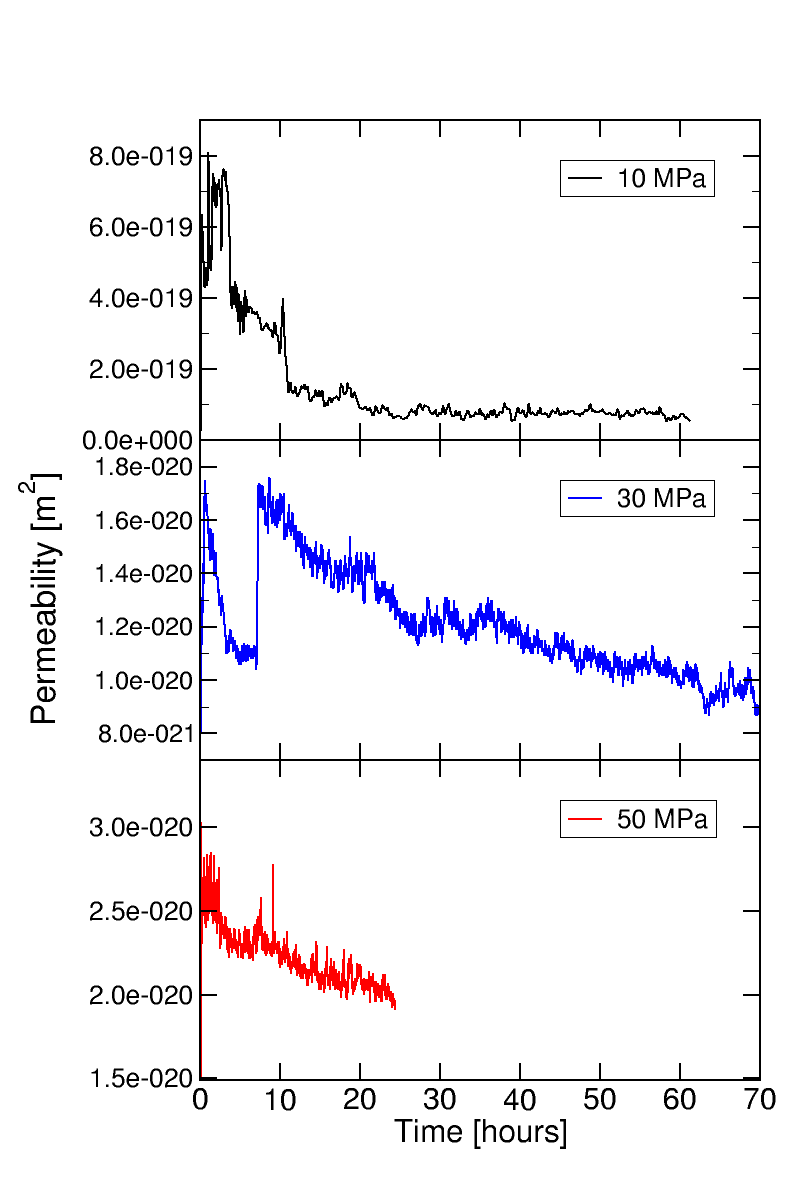
\includegraphics[width=0.75\textwidth]{figures/mex3-perme-time-comparison.png}
\caption{Graphical Representation of data}
\label{fig:dms-mex22-lab}
\end{figure}